\section{实验结果与分析}
% 一些关于序号的设置
\setcounter{figure}{0}
\subsection{训练时的损失敛散情况}
\begin{uscfigure}
	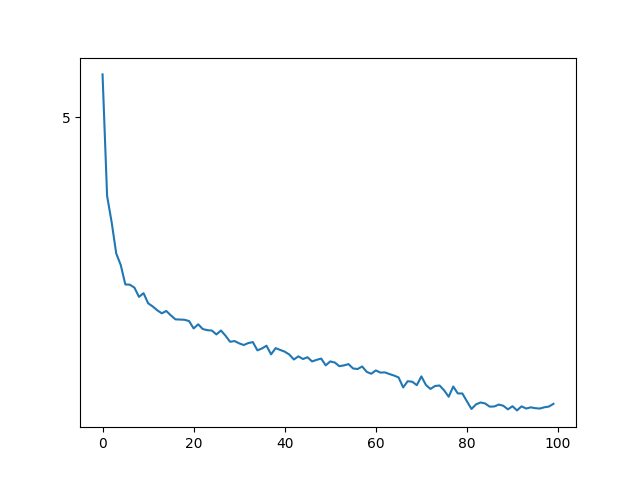
\includegraphics[width=\textwidth]{./Pictures/loss.png}	
	\caption{训练时的损失敛散情况}
	\label{loss}
\end{uscfigure}

本算法对8000张大小为224*224像素的图片进行了120000次迭代,如图\ref{loss}反映的是训练过程中的损失收敛的情况。横坐标中的1个单位表示的是1200次迭代,纵坐标的1个单位表示的是每1200次迭代的损失函数的平均值。
\subsection{改进SSD算法的实验结果}
\begin{uscfigure}
	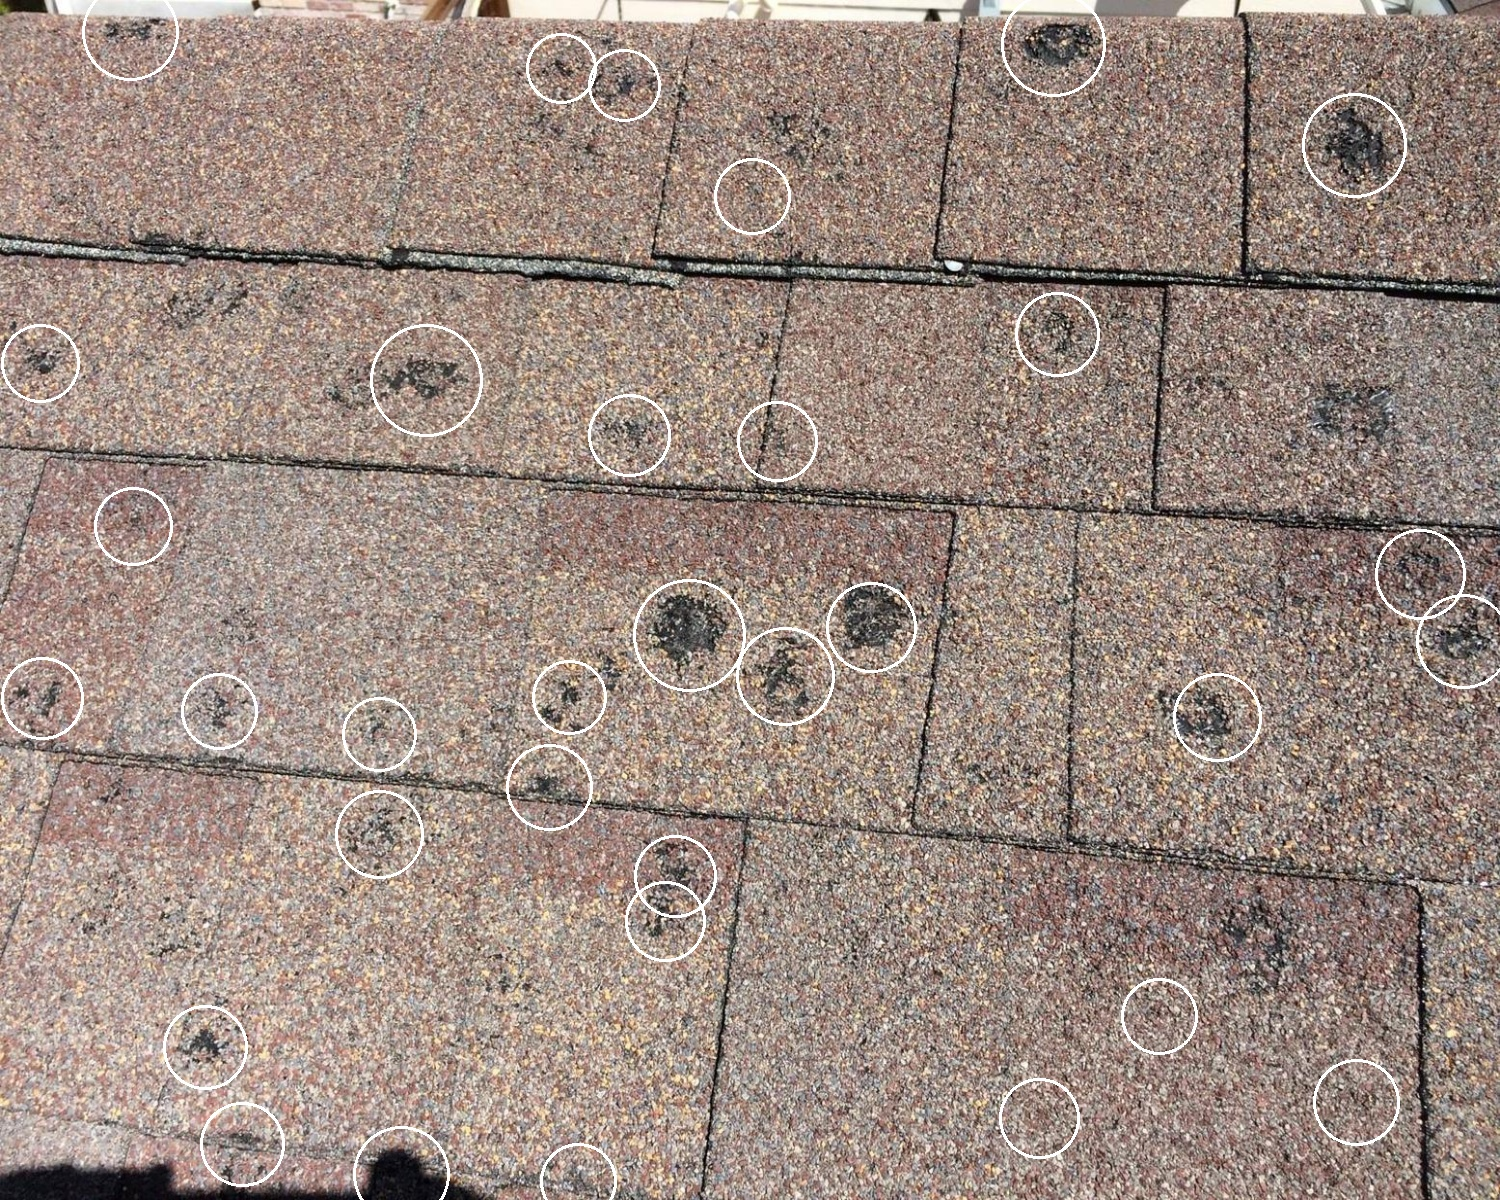
\includegraphics[width=\textwidth]{./Pictures/result.jpg}	
	\caption{检测结果}
	\label{result1}
\end{uscfigure}

从图\ref{result1}中可以看到形状如斑点的黑色区域就是瓦片被损害的区域,有大部分被检测出来了,但也有小部分没有检测出来,或者是被误检了。
\subsection{改进SSD对瓦片损害检测的准确率实验}
\begin{table}[htbp]
	\centering
	\caption{改进SSD算法的准确率及速度实验结果}
	\label{}
	\begin{tabular}{ccc}
		\toprule
		网络模型 & mAP & FPS\\
		\midrule
		SSD 	& 60\% & 90\\
		SSD+focal-loss  &  62\% & 87\\
		SSD+soft-nms & 64\% & 85 \\
		SSD+soft-nms+focal-loss & 65\% & 80\\
		\bottomrule
	\end{tabular}
\end{table}

mAP:Mean Average Precision 平均精度均值。

FPS:Frames Per Second 帧率
\subsection{实验结果分析}
从瓦片损害的检测实验过程中发现,其结果是低于原算法在PACSL VOC数据库中的实验结果的,其具体原因和以下几点:

1、瓦片损害的形态不定,且与距离受损害的时间的长短有关——时间越长损害处的颜色越深,不利于标注从而导致降低了算法的识别精度。

2、数据量不够导致了降低了识别精度,由于没有现成的房屋屋顶瓦片数据,且一般家庭住房不愿意无人机拍照。

3、相当数量的房屋屋顶年代久远,以至于瓦片自身已经风化,为检测任务添加了不确定性
\begin{uscfigure}
	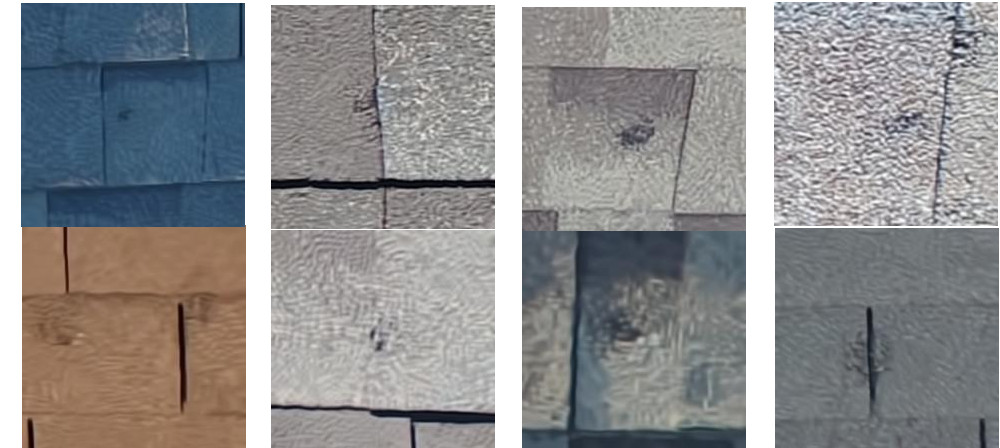
\includegraphics[width=\textwidth]{./Pictures/damage.jpg}	
	\caption{冰雹对瓦片造成的损害}
	\label{damage}
\end{uscfigure}
\subsection{算法改进建议}
随着目标识别相关算法的成熟,现在的识别精度已经超过了80\%,房屋瓦片损害检测只能充分利用其自身的特点,手工设计一些特征,从而提高算法的识别精度。与此同时,数据量是一个急需解决的问题,数据量一大,对于一些干扰就能有效的去除。
